\section{Remote 5 vs 5 gameplay}
\label{sec:OneVsOneChallenge}

\subsection{Idea of the competition}
% Patrick
The additional aim of this competition is to explore and demonstrate competitive remote gameplay given the current situation.

Two teams of each five robots (no substitute) play against each other on a full-sized (\cf section \ref{sec:field_dim}) standard robot soccer according to sligtly modified SPL 2022 rules in a remote arena (\cf section \ref{sec:Common_rules}). 

This competition differs from the standard RoboCup procedure in the following aspects:
\begin{itemize}
    \item Remote deployment with manual or fully autonomous setup of NAO software and standardized settings for game play in a remote arena on foreign robots,
    \item Automatic or semi-automatic calibration of NAO (vision, motion, etc.), 
    \item Safe operation of robots in gameplay without damaging robots,
    \item Operating a hosting arena for remote teams. 
\end{itemize}

\subsection{Prerequisites}
\label{sec:c3_Prerequisites}
% Patrick

\subsubsection{Basic requirements for teams}

Requirements to remotely participate in GORE 2022 are, being able to deploy your robot's software remotely or in a fully autonomous setup.

\subsection{Arena and organizational setup}
\label{sec:arean-org-setup}
% Patrick
This competition relies on a standardized arena setup as well as on exchanging all information necessary for gameplay. The following sections define the information used to describe local arena conditions.

\subsubsection{USB Drive}
\label{sec:c3_USB_Drive}
Tiny (not standing out the surface of the head like \url{https://www.amazon.com/dp/B077VXV323/}) USB drives remaining inside the head for the whole game are used to flash a robot with a binary image or to store data during the game play of the robot.

During the competition two kinds of USB drive are used. Their purposes are:

\paragraph*{Flashing}
This kind of USB Drive is used to flash a robot either with the standard SoftBank image or with a team provided one. After flashing, this USB Drive gets replaced by the \textit{storage} USB drive.

\paragraph*{Storage}
After \textit{Flashing} a robot, they will be equipped with a storage USB drive with ext3 file system. It will be used for the following purposes:

\begin{itemize}
	\item \textbf{Configuration}: Configuration files, at least \texttt{field\_dimensions.json} as explained below, will be copied into the root folder of the USB drive.
	\item  \textbf{Logging}: If teams want to store log files or images and get them uploaded in the Nextcloud as explained below, they can store the files in a \texttt{logs} folder on the USB-Drive.
\end{itemize}

\subsubsection{Data Exchange}
\label{sec:data_exchange}
Teams exchange data before and during GORE 2022 using a Nextcloud/Owncloud drive. An access link and password will be sent to the team leaders and have to be used with care. The network drive will contain a folder for every remote team according to their team number. Team folders will be used for sharing data. Example file structures are give in \ref{sec:file_structure}. 

\begin{itemize}
    \item In folder \textbf{field dimensions} the hosting arena has to provide a json file (template will be in the root folder of the drive) describing the field dimensions according to the rules (see \ref{sec:field_dim}). The file has to be named \texttt{field\_dimensions.json}. An example of this file you find in section~\ref{sec:fielddimensionsjson}. The file will be used for autonomous setup and game play. To configure the arena the corresponding field description will be copied in to the root folder of the USB drive, after flashing, as \texttt{field\_dimensions.json}. This allows the usage of the same image at different arenas.
    \item In \textbf{Robot Setup} the arena team finds a binary image for a particular game. Each game has an identifier \textit{Game\_ID} and this identifier has to be used as folder name. The binary image has to be uploaded \textbf{one hour} before the game starts. Next to the image you can define multiple configuration folders for each player. The containing files will be copied in the root on the USB drive. The USB drive will be plugged into the robot after flashing. Within this configuration folders you can also place files to configure your image. There is one mandatory file: \texttt{field\_dimensions.json}. This file has to be used by the robot's software.
    \item To allow an autonomous robot setup to identify the robot, both teams can upload after robot assignment (see \ref{sec:setup_two_hours}) a \texttt{robot\_id.json} into the corresponding folder of the team for the game. The \texttt{robot\_id.json} should have a structure to match \textbf{MAC-Address}, \textbf{IP} and \textbf{Robot ID}. An example is shown in Section~\ref{sec:robotidjson}.
    \item In the folder \textbf{field images} each hosting arena has a folder where photos from the arena from different angles and at different day \& night-times with focus on the lighting conditions are located.
    \item In \textbf{Arena Access} remote teams find an instruction how to access the arena. Each arena must provide team specific credentials and share them with the responsible person in each team. Every hosting team announces a responsible person for credentials and remote setup. The list of responsible people can be found in the root folder of the Nextcloud/Owncloud drive.
    \item In the hosting arena's root folder you find a \texttt{streaming.md} file where every hosting team has to publish a link that can be used by public to watch a game. Further details for streaming, see~\ref{sec:streaming_setup}.
	\item Logs and images will be uploaded from the hosts into the folder \texttt{<Team>/<Game\_ID>/Logs}, where \textit{Game\_ID} is replaced by the game identifier, after the game when bandwidth is available. It is assumed that logs and images are stored on the USB drive attached to the NAO in the folder \texttt{logs}. Other files will be ignored. For each robot a separate folder will be created to distinguish logs files from each robot. 
\end{itemize}

\paragraph{Example Nextcloud Storage File Structure}
\label{sec:file_structure}
\ \\
    \begin{forest}
        for tree={font=\sffamily, grow'=0,
        folder indent=.9em, folder icons,
        edge=densely dotted}
        [root
            [HULKs \%fully automated setup with own binary and with hosting an arena
                [arena
                    [arena1..10.jpg, is file]
                    [arena\_access.md, is file]
                    [streaming.md, is file]
                    [field\_dimensions.json, is file]
                    [robot\_network\_identification.csv, is file]
                ]
                [games
                    [1 \%Game\_id
                        [image.bin, is file]
                        [configuration
                            [field\_dimensions.json \%mandantory, is file]
                            [robot\_id.json, is file]
                            [game\_configuration.json, is file]
                        ]
                        [logs
                            [many\_many\_files.files]    
                        ]
                    ]
                ]
            ]
            [NAO Devils \%semi automated setup using SBR image and no arena
                [games
                    [1 \% Game\_id
                        [configuration
                            [field\_dimensions.json \%mandantory, is file]
                        ]
                        [logs]
                    ]
                ]
            ]
        ]
    \end{forest}


\paragraph{Example USB Stick File Structure}
\ \\
    \begin{forest}
        for tree={font=\sffamily, %grow'=0,
        folder indent=.9em, folder icons,
        edge=densely dotted}
        [root
            [field\_dimensions.json, is file]
            [further\_config\_files.files, is file]
            [logs]
        ]
  \end{forest}


\subsubsection{Network Setup}
The following section defines network requirements for hosting remote games. The network infrastructure should be as transparent as possible for remote participants. It should get as close as possible to an on-site experience. Please also contact your local IT administrators and agree your setup with them.

\paragraph{General}

\begin{itemize}
    \item Participants need easy access to their robots for uploading code and debugging. No ports should be blocked. ICMP must not be blocked. % TODO: Which ports are necessary?
    \item Robots might accumulate a large amount of log files (including images). These logs will be uploaded after games for analysis. Minimum 100Mbit/s (symmetric) is recommended for a venue, favourable 1Gbit/s. Logs can also be uploaded from another network.
    \item To not overwhelm the network, teams should rate limit their network activity (in particular long log downloads and uncompressed video streams from NAOs during debug sessions)
\end{itemize}

\paragraph{SPL Game specific}

\begin{itemize}
    \item Team Messages (SPLStandardMessages) must be receivable for remote participants.
    \item Team Messages must not be forwarded from remote participants to 10.0.0.0/16 (SPL\_A).
    \item GameControllerMessages must be receivable for remote participants.
    \item GameControllerMessages must not be forwarded from remote participants to 10.0.0.0/16 to not allow remote participants to control the game (by accident).
\end{itemize}

\paragraph{Example configuration}
\label{sec:example_configuration}

\begin{figure}[ht!]
    \centering
    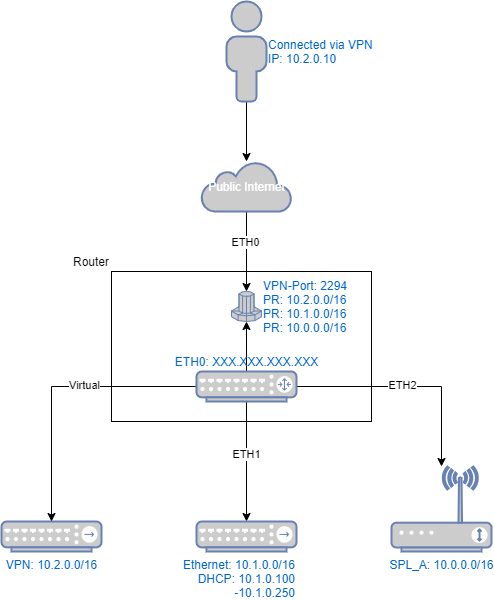
\includegraphics[width=0.5\textwidth]{figs/network.png}
    \caption{Network setup example}
\end{figure}

\begin{itemize}
    \item  The network could be divided for example into three subnets:
    \begin{itemize}
        \item 10.0.0.0/16: The actual SPL\_A wifi network on at least 2.4\,GHz. Each team must use 10.0.TEAM\_NO.2-254 for their robots. GameController will be on 10.0.0.2. DHCP is not active.
        \item 10.1.0.0/16: The ethernet network for robots. Each team must use 10.1.TEAM\_NO.2-254 for their robots. Static addressing is required when robots are assigned to a team. DHCP is active, statically assigning 10.1.0.2-255 to robots that are currently not assigned to any team (pool).
        \item 10.2.0.0/16: The VPN network. Remote participants are assigned to this network and can access the other networks. Team- and GameControllerMessages are forwarded from 10.0.0.0/16 to this subnet. DHCP is active. Broadcasting to other subnets is not possible.
    \end{itemize}
    \item Router (e.g. Ubiquiti EdgeRouter Lite 3-Port Router from Ubiquity \url{https://www.ui.com/edgemax/edgerouter-lite/})
    \begin{itemize}
        \item serves as router for the whole network.
        \item assigns static IPs for flashed robots based on their MAC-address
        \item has a globally routable (and accessible) IPv4 address.
        \item hosts an OpenVPN Layer2 VPN Server
        \item opens a network port to allow incoming OpenVPN connections
        \item Every team gets one certificate to authenticate via OpenVPN (multiple connections allowed).
        \item Has broadcast forwarding rules in place to allow VPN users to receive Team-/GC-Messages.
        \item GameController computer is assigned 10.0.0.2/16
        \item \texttt{ETH0} could be connected to your university network and is preferably accessible from the internet on the specific port (please contact your computer center how to realize such a connection). If this is not possible, please check if you can make this network accessible from remote using a mobile internet connection. Or you provide a PC connected to an island network of this structure where people can access the PC using TeamViewer, remote desktop software, or something similar. 
    \end{itemize}
    \item Automated assignment of IP address to robots after being flashed.
    \begin{itemize}
        \item \label{sec:robot_table} The hosting arenas prepare a file \texttt{robot\_network\_identification.csv} with the following columns: [Robot ID, Team, Team Identifier (Name written on the robot), Head ID, Body ID, MAC address of LAN, IP-Lan address]
        \item Each team will fill in the data (Except IP Addresses) into the table for its robots.
        \item Each hosting team verifies this data when robots arrive.
        \item Each hosting team assigns static IP addresses to the robots based on the data in the table and lists the IP address there.
        \item This address can than be used by the teams to take over the robot after flashing. The Address has to be changed during configuration.
    \end{itemize}
\end{itemize}

If you have questions or problems to set your local network, please contact the organisers via email. There will be also a Discord channel for networking to share configuration files and to solve problems.

\subsection{Remote \& Game Setup}
\label{sec:remote_game_setup}
This section describes the setup procedure for a 5 vs. 5 match. The setup procedure distinguishes between fully-autonomous and semi-autonomous setup. The used setup procedure is not relevant for scoring the game.

\subsubsection{Button Interface}
To give volunteers an interface to command autonomous acting robot, new game states and button interface sequences have been introduced (see \ref{sec:robot_states}).

\subsubsection{Start: 1h before match}
\label{sec:setup_two_hours}

    \begin{enumerate}
        \item Assignment of a volunteer (are also assistant referees in the game) from the host team for each remote team. They create own Discord rooms for communication during the whole setup and game phase and communicate this to the teams.
        \item Initial meeting of the volunteers and the representatives from the teams in one of the Discord rooms.
        \item Topics of this meeting are: Welcome, answering questions, agree on timing for calibration, and selecting robots, selection of jerseys.
		\item For each team five randomly (see next points) selected functional robot are assigned from the pool.
		\begin{enumerate}
            \item The host team has a numbered list of functional robots from 1 to the maximum number.
            \item One volunteer screen shares a proper random number generator (\url{https://www.random.org/integers/}) with adjusted settings according to the number of available robots.
            \item The volunteer runs the number generator. The first valid number is the robot number for the home team, away team is second. Third number is the second robot for the away team and fourth for home team. They continue until each team got 5 robots assigned. 
            \item If a robot, who wears the selected number, is already taken or not available, than the generator has to be run again. 
        \end{enumerate} 
        \item Move to the individual Discord rooms to shortly discuss the team specific setup, robot jersey number assignement, calibration and game play procedure with the volunteer. Teams and volunteer will use this room for the reminder of setup and game. And stay connected through this. Also in the game play phase when they are assistant referees.
        \item The competing team informs the competition venue if they are using fully-autonomous or semi-autonomous setup.
        \item The competing team finalizes the content of the \texttt{Game\_ID} folder in the Nextcloud. At least copy the \texttt{field\_dimensions.json} of the arena to the respective configuration folder.
        \item Connect the robot (should already be fully charged) to a charger. If the competing team chose semi-autonomous setup, a LAN cable is connected as well.
        \item Each robot gets flashed 
        \begin{itemize}
            \item with the standard SoftBank binary image or
            \item with the image provided by the respective team.
		\end{itemize}
		\item Each robot gets equipped with a USB drive according to \ref{sec:c3_USB_Drive} (Assistants please check) and started.
        \item Teams can set their robot up remotely, if necessary. To reduce the amount of data transferred to set the robot up, teams should reduce this as much as they can and use installable images where possible. If the competing team chose fully-autonomous setup, this step is skipped.
        \item The IP address given by the DHCP Server is static and their addresses are available in the Nextcloud/Owncloud folder (see \ref{sec:example_configuration}). If the competing team chose fully-autonomous setup, this step is skipped.
        \item According to the official game schedule, the first team named is the home team, plays on the left half of the field and the second called team is the away team and play on the right half of the field from the perspective of the GameController. 
        \item Dress robots with jerseys (see \ref{sec:team_markers}). By default: The hosting team's 'home' and 'away' jersey are assigned to the 'home' and 'away' starting robots, respectively. If a team wants to use its own jerseys they have to send the home jerseys to their primary arena and they can also send their away jerseys to the other arena. Validate that the robots wear the correct jerseys using for example the GameController.
    \end{enumerate}

\subsubsection{Calibration / Testing: at least 30 minutes before match}
    \begin{enumerate}
        \item 30 minutes to calibrate the robots supported by one volunteer.
        \item All robots than can move over their half of the field, except into the centre circle, to calibrate themselves. The volunteers have to actively watch the robots and to be ready to catch one as soon as it would leave the field or fall. The volunteers are allowed to catch robots. To prevent damage the same rules as in normal game play have to be applied to prevent damage to the robots (see \ref{sec:forbidden_act}).
        \item Before the calibration starts, at the middle of each line connecting penalty spot and the center of the center circle a ball gets placed. The robots can move their ball. If a ball leaves the field, it gets replaced at its kick-in position (see \ref{sec:kick_in}). If a robot scores a goal, the ball gets moved back to its starting position. If the ball moves to the opponent's half, it is out.
        \item \textbf{Automatic calibration} is conducted in the following way: The volunteer places the robots on the normal initial positions (see Fig.\,\ref{fig:initial_positions}) at the field side of a field. Then the volunteer presses button to get the robots into calibration state~(see~\ref{sec:robot_states}). At the end of the calibration period, the robot may sit down and get unstiffed by the volunteer. Otherwise, the robot will be unstiffed by the volunteer by pressing all head buttons simultaneously~(see~\ref{sec:robot_states}). Best is to run calibration for each robot separately. This procedure should be agreed between assistant and team, if all robots at the same time, or after each other, or ... are in the calibration phase.
     
        \textbf{Semi-automatic calibration}: With support of a local volunteer the robots are calibrated remotely. Both volunteer and remote team meet in a Discord room and perform the calibration procedure of the remote team together.

        \item  Check Wi-Fi and game controller connection
    \end{enumerate}

\subsubsection{Game Setup}

	\begin{enumerate}
		\item Robots are in the game controller
		\item Robots are placed according to Section~\ref{sec:kick-off}.
		\item The game will be started using the game controller as \textit{Play-off game} and the robot moves to its starting position.
		\item In \texttt{Set} the balls will be placed and the game will be started using a whistle.
		\item In the second half the robots switch their sides.
		\item Referees apply rules with focus on preventing hardware damage, because there is no SoftBank Robotics support (see \ref{sec:forbidden_act}).
		\item When robots receive the finish message they have to sit down and will be brought to the chargers and plugged into network.
	\end{enumerate}
	
\subsubsection{After Game}
	
	\begin{enumerate}
		\item After robots received the finish state of the second half of the game controller they have to sit down.
		\item Robots have time to do all post-processing, storing the logs and shutting down.
		\item If robots are not switched off after 5 minutes they will be switched off manually.
		\item The data from the USB drive will be stored on another device and as soon as possible uploaded in the Nextcloud/Owncloud.
		\item Teams are not allowed to download their logs directly.
		\item Robots will be returned to pool for the next game.
	\end{enumerate}

\subsection{field\_dimensions.json example}
\label{sec:fielddimensionsjson}

\begin{lstlisting}[language=json,firstnumber=1]
{
    "field": {
        "length": 9.0,
        "width": 6.0,
        "lineWidth": 0.05,
        "penaltyMarkerSize": 0.1,
        "goalBoxAreaLength": 0.6,
        "goalBoxAreaWidth": 2.2,
        "penaltyAreaLength": 1.65,
        "penaltyAreaWidth": 4.0,
        "penaltyCrossDistance": 1.3,
        "centerCircleDiameter": 1.5,
        "borderStripWidth": 0.7
    },
    "goal": {
        "postDiameter": 0.1,
        "height": 0.8,
        "innerWidth": 1.5,
        "depth": 0.5
    }
}
\end{lstlisting}


\subsection{robot\_id.json example}
\label{sec:robotidjson}

\begin{lstlisting}[language=json,firstnumber=1]
{
    "12-34-56-78-9A-BC": {
        "player": 1,
        "IP": "10.0.TEAM_NO.11"
    },
    "12-34-56-78-9A-AF": {
        "player": 2,
        "IP": "10.0.TEAM_NO.12"
    }
}
\end{lstlisting}

\subsection{Common rules}
\label{sec:Common_rules}
The 5 vs. 5 games played at the GORE 2022 are designed to use the rules of RoboCup SPL. However, to facilitate the remote participation of all teams and the common robot pool, various changes are required.

Therefore, the following re-produces the current draft of rules for the RoboCup SPL 2022, with various details that have been modified, added and/or omitted. All changes are marked with a \cbw{colourbox} and a list of major rule changes can be found in Section~\ref{sec:major_rule_changes}.

\subsubsection{Major Rule Changes}
\label{sec:major_rule_changes}
\begin{itemize}
\item Only NAO V6 is allowed, \cf Section~\ref{sec:hardware}.
\item Requiring of a streaming setup for a host arena, \cf Section~\ref{sec:streaming_setup}.
\item Each team obtains 5 robots from a robot pool but there will be no replacement of robots, \cf Section~\ref{sec:field_players} and Section~\ref{sec:game_struct}! \cbw{(Maybe relaxed in the first teamleader meeting)}
\item Each robot in a robot pool gets a unique ID and for this purpose stickers can be placed on the upper arms and the back of the head, \cf Section~\ref{sec:robot_pool_markers}.
\item For teams that are not on site, the assistant referees take over tasks as if they were a member of the corresponding team, \cf Section~\ref{sec:request_for_pickup}, Section~\ref{sec:request_for_timeout}, Section~\ref{sec:penalty_shoot-out} and Section~\ref{sec:assist_referee}.
\item Goalkeepers are only allowed to dive during a penalty kick, \cf Section~\ref{sec:forbidden_act}, Section~\ref{sec:penalty_free_kick} and Section~\ref{sec:penalty_kick}. \cbw{(Maybe relaxed in the first teamleader meeting)}
\item For teams that are playing with robots from other teams, there is a maximum of two hardware related penalties for each robot in the first half and one more in the second half, \cf Section~\ref{sec:forbidden_act}. \cbw{(Maybe relaxed in the first teamleader meeting)}
\item The head referee decides whether a robot excessively damages itself and removes it from the field via ``Request for Pick-up'', \cf Section~\ref{sec:damage_robot}.
\item All referees are allowed to prevent robots from crashing to the ground by catching them beforehand and then laying them down gently, \cf Section~\ref{sec:damage_robot} and Section~\ref{sec:judgment}. \cbw{(Maybe relaxed in the first teamleader meeting)}
\item Fallen robot penalty: A robot has a maximum number of two attempts (or in exceptional cases 3) to get up and has to be at least 10 seconds upright, \cf Section~\ref{sec:fallenrobots}.
\item Pushing may occur between any robots, \ie also between team mates, \cf Section~\ref{sec:player_pushing}. \cbw{(Maybe relaxed in the first teamleader meeting)}
\end{itemize}